\chapter{Обсуждение результатов} \label{chapt5}

\section{Инвариантные спектры по поперечному импульсу} \label{sect5_spectra}

Форма полученных \pt-спектров зависит от типа частиц. В логарифмическом масштабе инвариантные \pt-спектры \pipm - мезонов вогнуты внутрь, инвариантные \pt-спектры \Kpm - мезонов имеют прямую форму, а инвариантные \pt-спектры \prot \ и \aprot \ выпуклые наверх.
Данное различие в формах \pt-спектров заряженных адронов может быть количественно интерпретировано путем перехода к спектрам по поперечной массе   $m_T = \sqrt{m_{0}^{2} + p_{T}^{2}}$, где $m_0$ - масса адрона. 

В диапазоне поперечных масс $m_T-m_0$~$<$~1.5~ГэВ инвариантные \mt-спектры могут быть описаны в рамках модели гидродинамики и  аппроксимированны следующей функцией:
\begin{equation}
	\label{eq:spectra_mt}
	\frac{1}{2\pi m_T} \frac{d^2 N}{dm_T dy}=\frac{1}{2\pi T (T+m_0)}\cdot A \cdot exp \left( -\frac{m_T - m_0}{T}\right)
\end{equation}


%Модели гидродинамики описывают спектры заряженных адронов в центральных столкновениях в диапазоне \pt~$<$~1.5~ГэВ/с. Однако, эти модели оказываются несостоятельными при описании периферических столкновений и при описании спектров в области \pt~$>$~2~ГэВ/с. 

Инвариантные спектры по поперечному массе, измеренные для положительно и отрицательно заряженных адронов в различных центральностях p+Al, \heau, Cu+Au и U+U столкновениях представлены на рис. \ref{img:SpectraMt0}, \ref{img:SpectraMt1}. Аппроксимация спектров с помощью формулы \ref{eq:spectra_mt} изображена черными прямыми линиями.

\begin{figure}[] 
	\centerfloat
	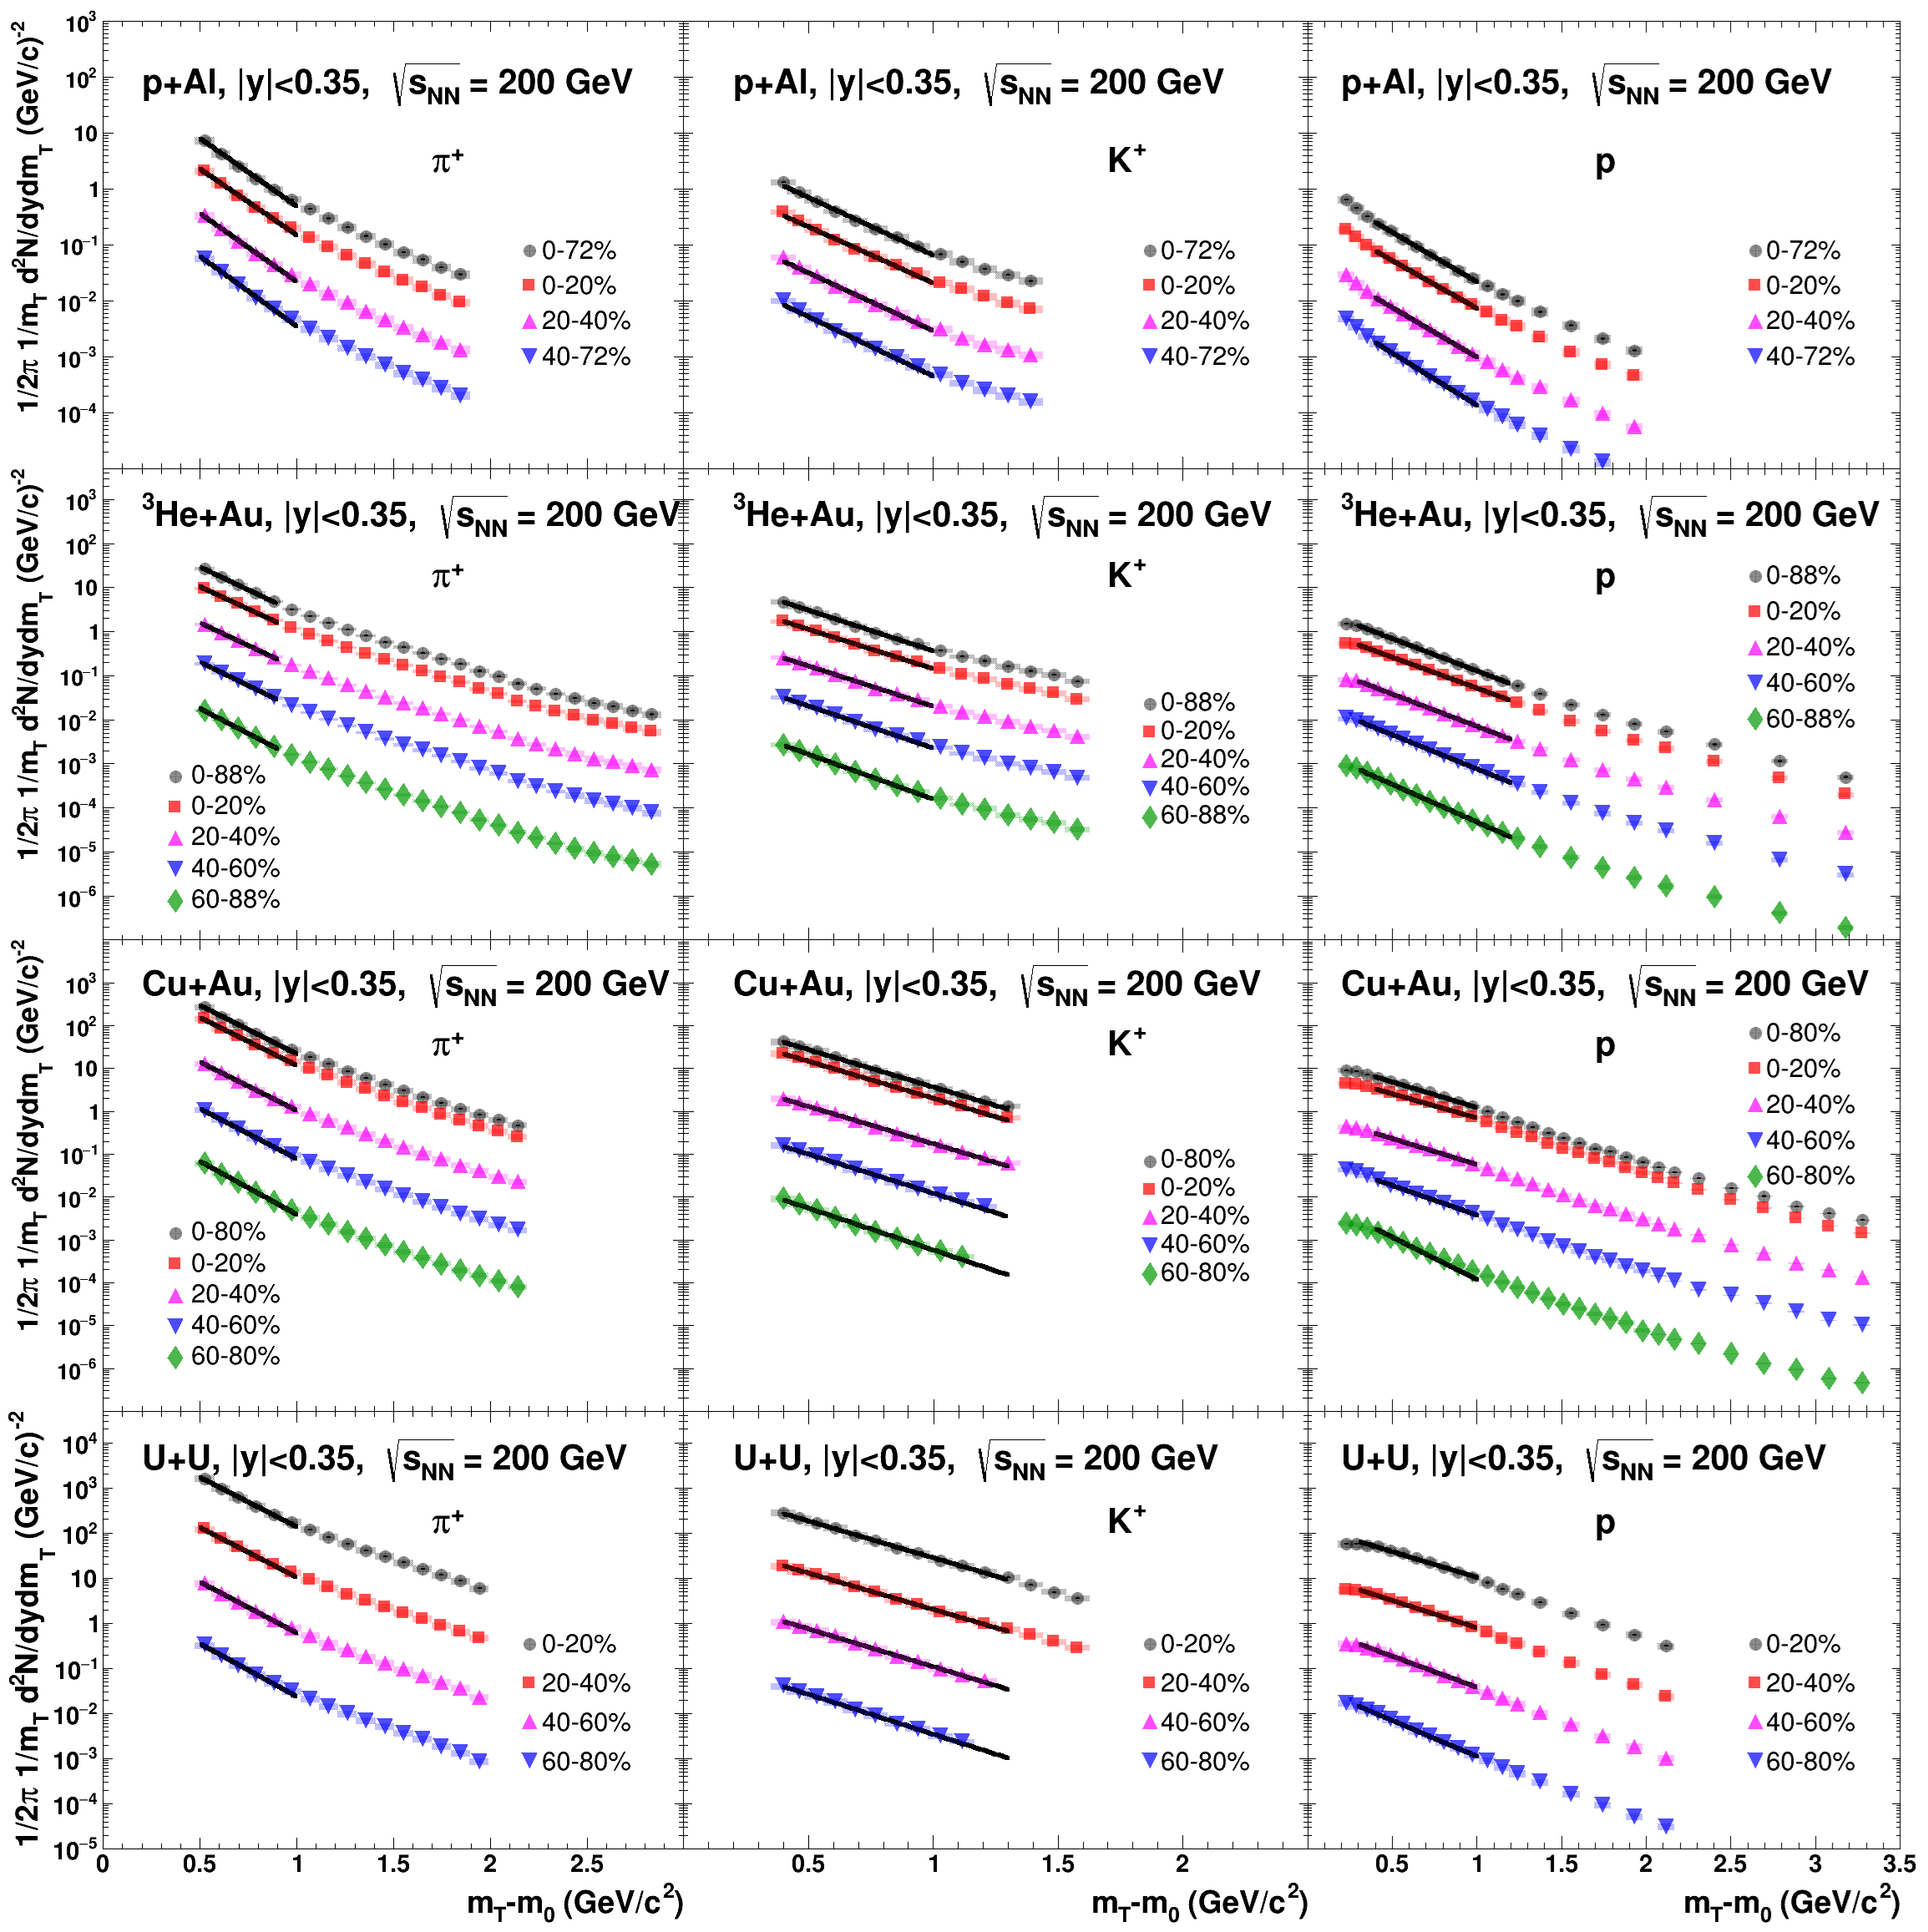
\includegraphics [width=1\linewidth]{Results/spectraDiss_mt_0.png}
	\caption{Инвариантные спектры по поперечному массе, измеренные для положительно заряженных адронов в различных центральностях p+Al, \heau, Cu+Au и U+U столкновениях.} 
	\label{img:SpectraMt0}
\end{figure}
\begin{figure}[] 
	\centerfloat
	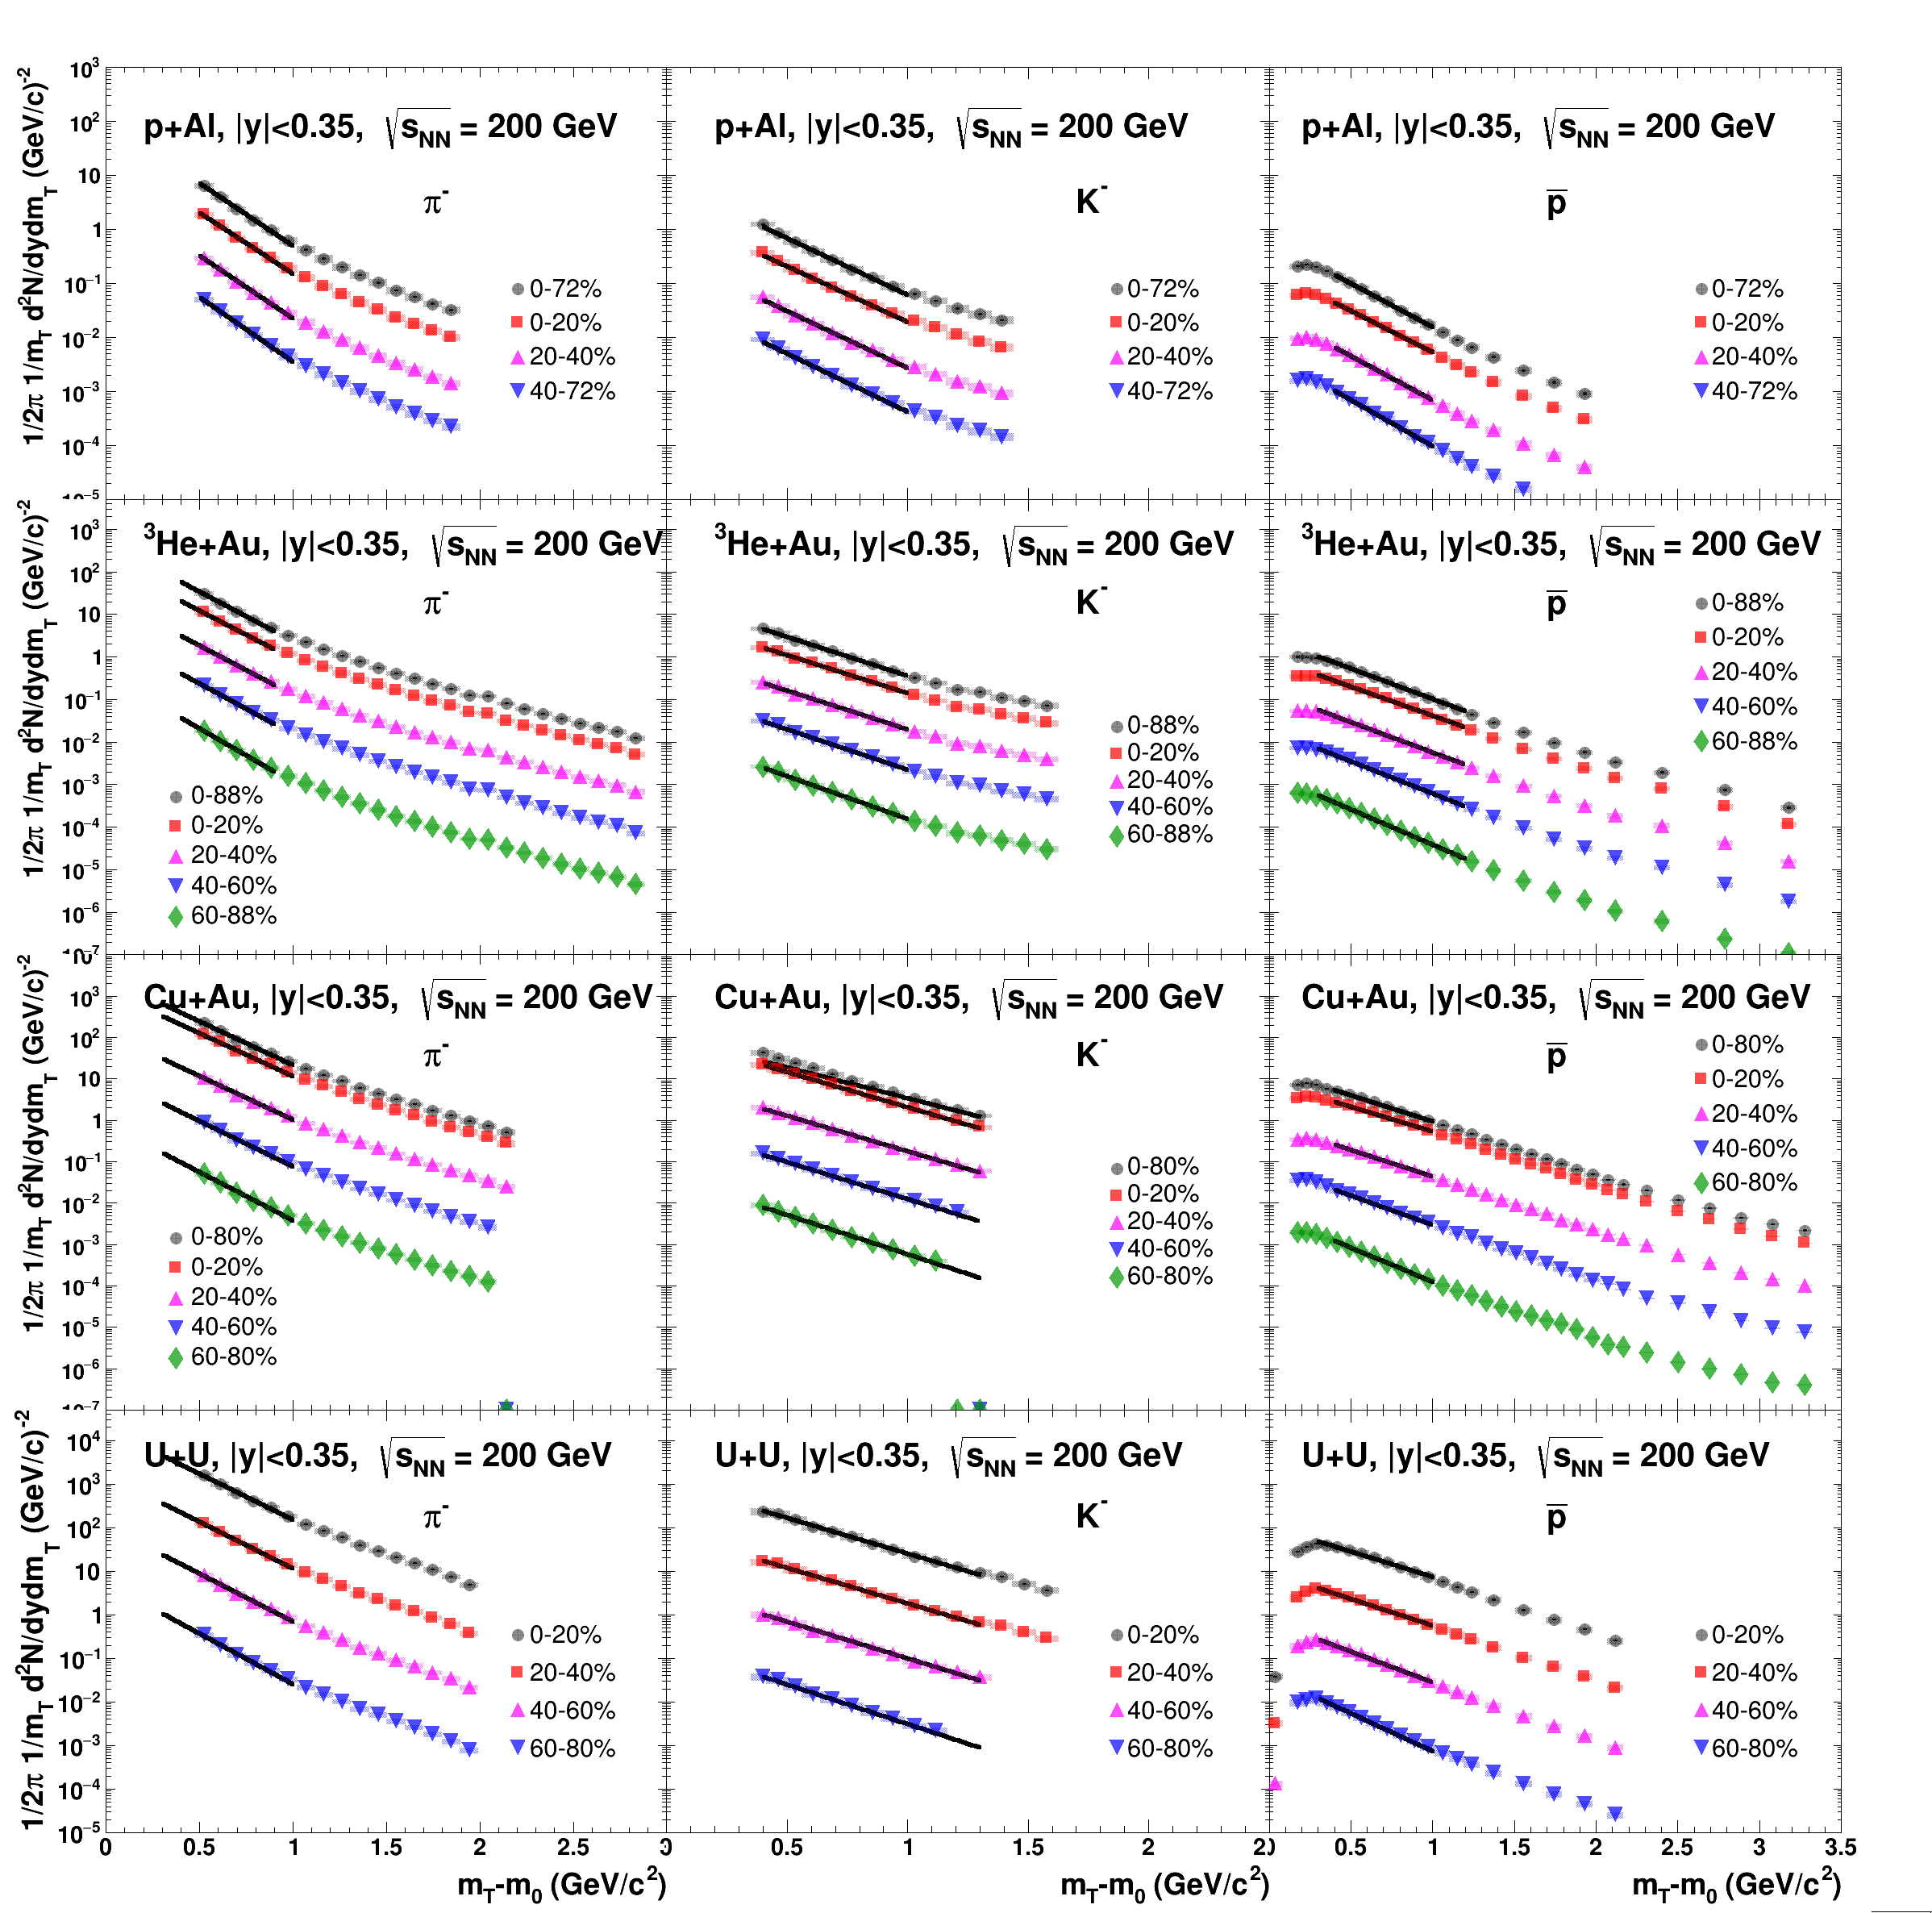
\includegraphics [width=1\linewidth]{Results/spectraDiss_mt_1.png}
	\caption{Инвариантные спектры по поперечному массе, измеренные для отрицательно заряженных адронов в различных центральностях p+Al, \heau, Cu+Au и U+U столкновениях.} 
	\label{img:SpectraMt1}
\end{figure}

Полученные параметры обратного наклона аппроксимационных прямых ($T$) представлены на рис. \ref{img:Tinv0}, \ref{img:Tinv1} как функция массы положительно и отрицательно заряженных адронов в различных интервалах центральности столкновений p+Al, \heau, Cu+Au, U+U. Значения параметров $T$ увеличиваются с увеличением массы частиц во всех рассматриваемых инервалах центральности во всех рассматриваемых системах столкновений.  
Согласно моделям гидродинамики, система находится в термическом равновесии, а частицы приобретают дополнительную компоненту скорости $\left< u_t \right>$, возникающую благодаря движению коллективного потока. При температуре $T_{0}$ частицы перестают взаимодействовать друг с другом, т.е. наступает так называемое кинетическое вымораживание. 
Данные зависимости $T$($m$) могут быть аппроксимированы линейной функцией с параметрами \To и \ut:
\begin{equation}
	\label{eq:InvSlope}
	T = T_0 +m \left< u_t\right>^2
\end{equation}
где $T$ - температура при которой достигается химическое равновенисие КГП, \ut - поперечная скорость коллективного движения партонов. 
Зависимость параметров обратного наклона $T$ от массы положительно и отрицательно заряженных адронов представлена на рис. \ref{img:Tinv0}, \ref{img:Tinv1}.
Полученные значения параметров аппроксимации приведены в таблицах приложения \ref{AppendixB}.

\begin{figure}[] 
	\centerfloat
	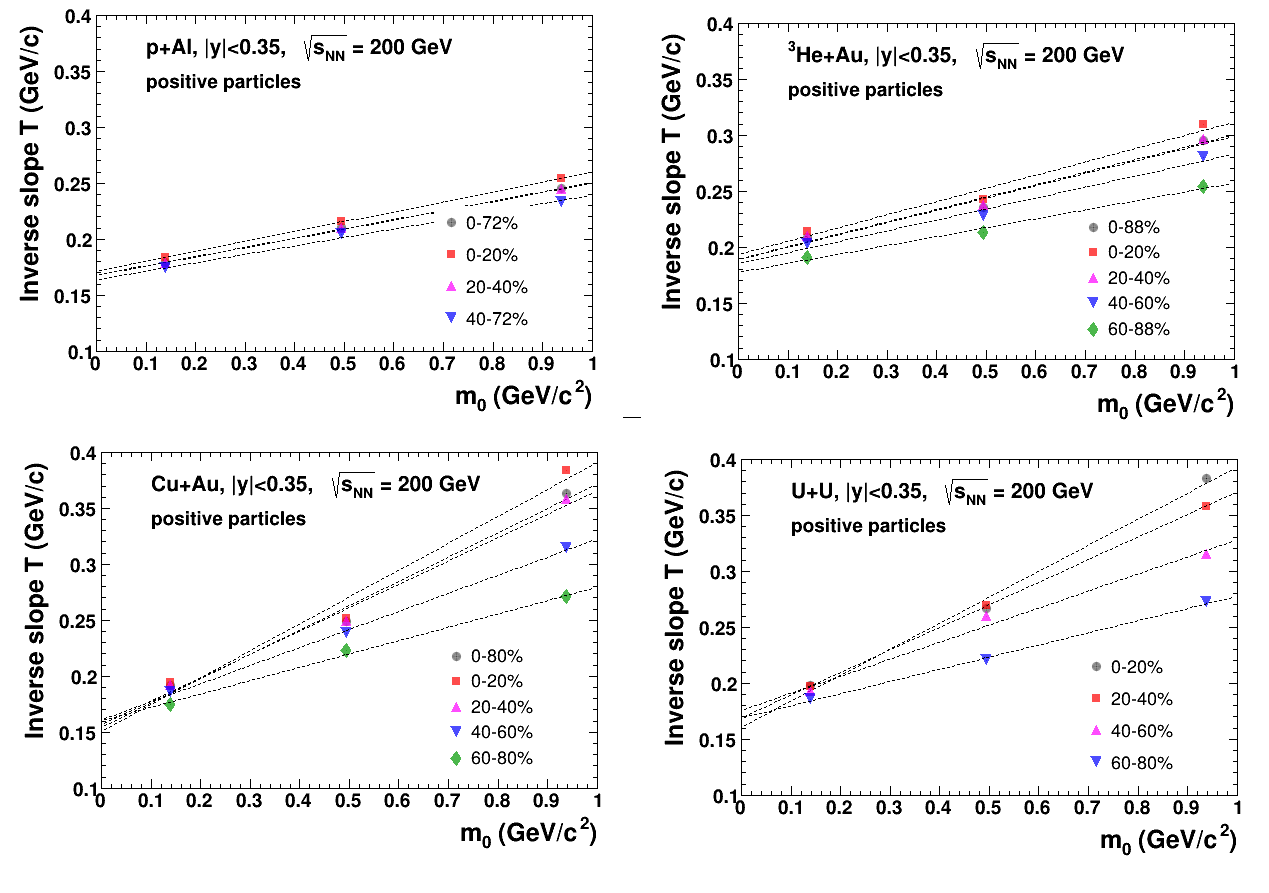
\includegraphics [width=0.7\linewidth]{Results/Tgr0.png}
	\caption{Зависимость величины параметра обратного наклона $T$ от массы \pip, \Kp, \prot в различных центральностях p+Al, \heau, Cu+Au и U+U столкновениях.} 
	\label{img:Tinv0}
\end{figure}
\begin{figure}[] 
	\centerfloat
	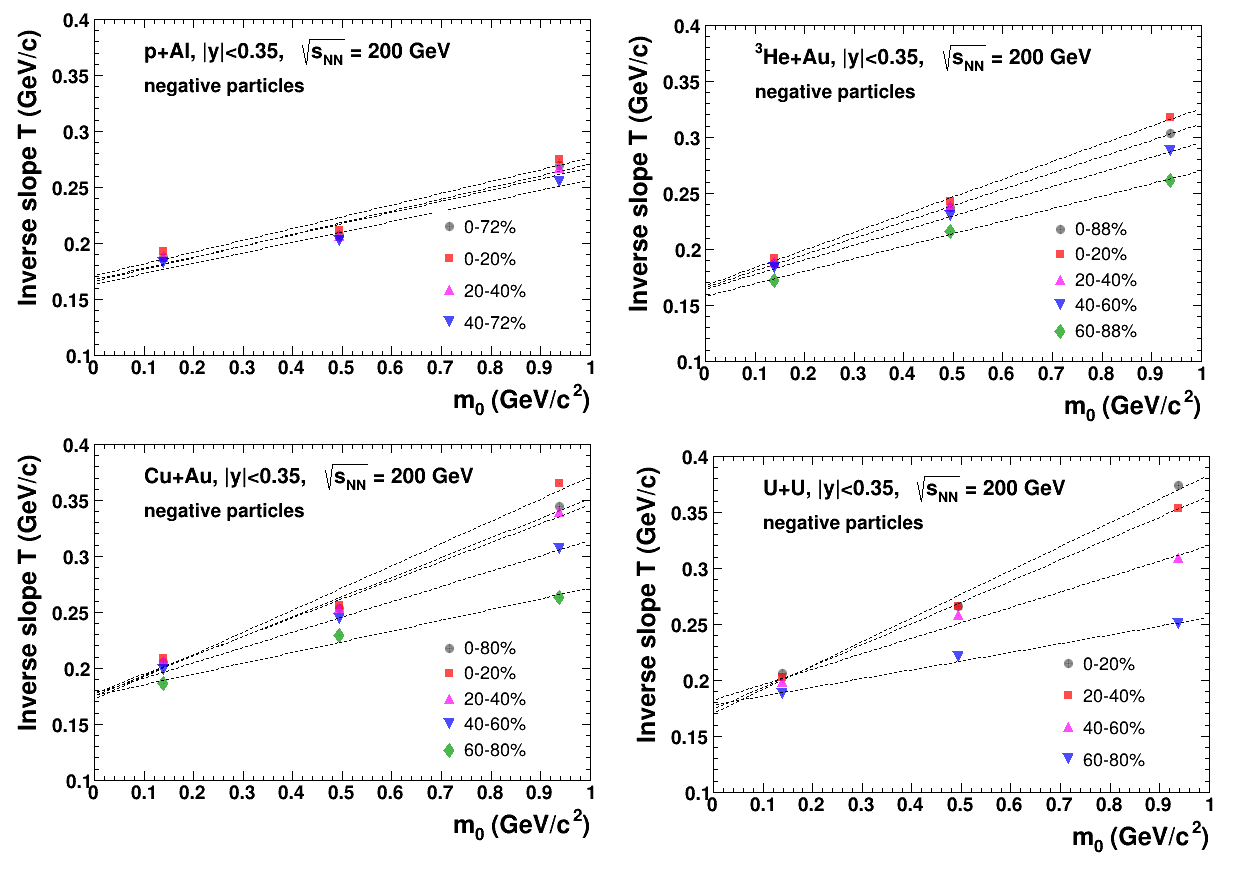
\includegraphics [width=0.7\linewidth]{Results/Tgr1.png}
	\caption{Зависимость величины параметра обратного наклона $T$ от массы \pim, \Km, \aprot в различных центральностях p+Al, \heau, Cu+Au и U+U столкновениях.} 
	\label{img:Tinv1}
\end{figure}

Линейная аппроксимация зависимости $T(m_0)$ с использованием уравнения. \ref{eq:InvSlope} изображена на рисунках \ref{img:Tinv0}, \ref{img:Tinv1} пунктирными линиями. Полученные значения $T_0$ и $\left< u_t \right>$ приведены в таблице приложения \ref{AppendixB} и представлены на рис.\ref{fig:TuNpart} как функция значений \Npart. Во всех рассматриваемых системах значения $T_0$, которые можно интерпретировать как линейную экстраполяцию параметра наклона $T$ к нулевой массе, имеют одинаковые значения во всех классах центральности, что может быть интерпретировано как независимость температуры вымораживания от центральности. С другой стороны, значения $\left< u_t \right>$ увеличивается с ростом центральности, что находится в соответствии с гидродинамической картиной.


\begin{figure}[ht]
	\centerfloat{
		\hfill
		\subcaptionbox{ }{%
			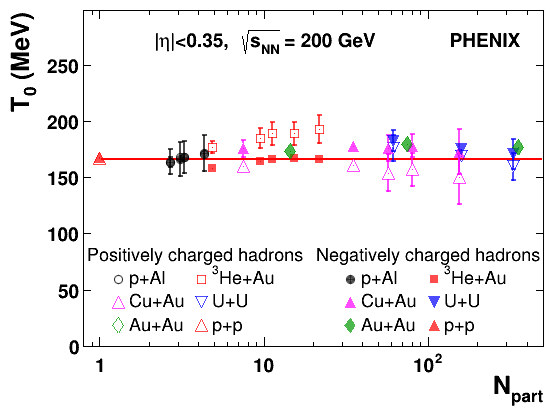
\includegraphics[width=0.45\linewidth]{Results/T0_Npart.png}}
		\hfill
		\subcaptionbox{ }{%
			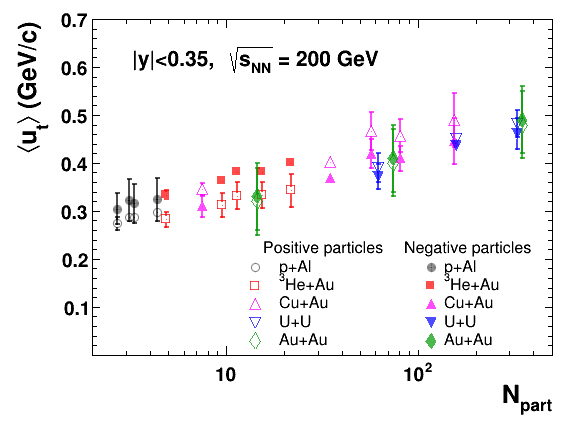
\includegraphics[width=0.45\linewidth]{Results/ut_Npart.png}}
		\hfill
	}
	\caption{Зависимость а) температуры вымораживания $T_0$ и  б) скорости поперечного потока $u_T$ от количество нуклонов участников \Npart.}\label{fig:latex}
\end{figure}

Коллективное движение, характеризуемое параметром \ut, обычно связывают с признаками образования КГП. В этом случае зависимость параметров \To и \ut от значений \Npart \ вместе с различными признаками образования КГП может быть важна для понимания минимальных условий формирования КГП.

\section{Сравнение с результатами моделирования} \label{sect5_spectra}